\section{Transactional Systems}
\url{../other/professor's slides/1_Transactions_NEW.pdf}\newline
\newline
A \textbf{transaction} is an elementary, atomic, unit of work performed by an application.\newline
Each transaction is conceptually encapsulated within two commands:
\begin{itemize}
    \item \textbf{begin of transaction} (bot);
    \item \textbf{end of transaction} (eot).
\end{itemize}
Within a transaction, \textbf{one} of the commands below is executed (\textbf{exactly once}) to signal the end of the transaction:
\begin{itemize}
    \item \textbf{commit};
    \item \textbf{rollback}.
\end{itemize}
\ \newline
\textbf{Transactional System} (OLTP) is a system that supports the execution of transactions on behalf of concurrent applications.\newline
\newline
A transaction is a unit of work enjoying the \textbf{ACID} properties:
\begin{itemize}
    \item \textbf{Atomicity} (abort-rollback-restart, commit protocols): either all the operations in the transaction are executed or none is executed;
    \item \textbf{Consistency} (integrity checking of the DBMS): a transaction must satisfy the DB integrity constraints, if the initial state is consistent then the final state is also consistent, but this is not necessarily true for the intermediate states of the transaction;
    \item \textbf{Isolation} (concurrency control): the concurrent execution of a number of transaction must produce the same result as the execution of the same transactions in a sequence;
    \item \textbf{Durability} (recovery management): the effect of a transaction that has successfully committed will last "forever".
\end{itemize}
\ \newline
Lets take a look at where are the ACID properties managed in the DBMS architecture:
\begin{center}
    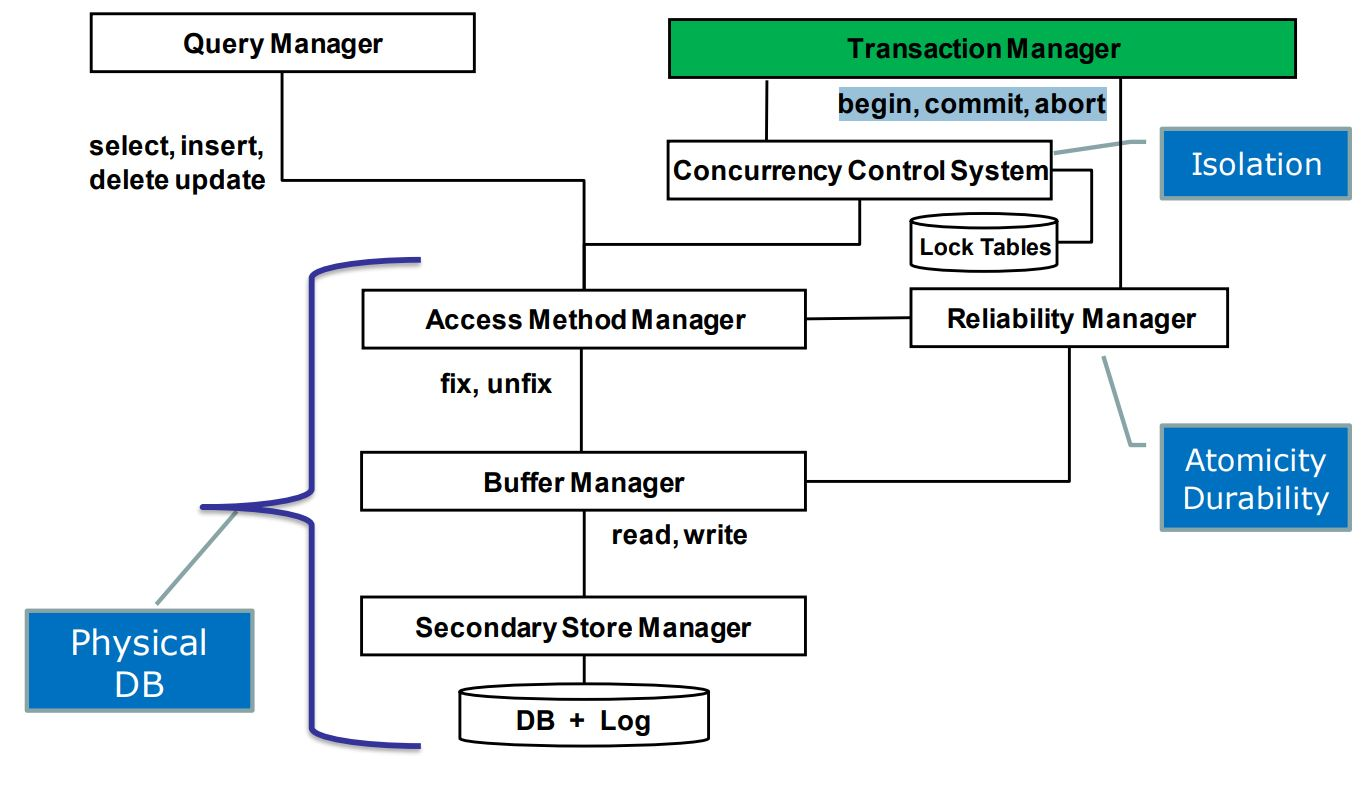
\includegraphics[height=7cm]{../arguments/ACIDandDBMSarchitectures.JPG}
\end{center}
